\documentclass[12pt, a4paper]{article}
\usepackage[utf8]{inputenc}
 
\usepackage{listings}
\usepackage{color}
\usepackage{graphicx}
\usepackage{geometry}
\usepackage{amssymb}
\usepackage{amsmath}
\usepackage{tcolorbox}
\usepackage{enumitem}
\usepackage{float}
 
\geometry{
 a4paper,
 left=20mm,
 top=20mm,
 bottom=20mm
 }
\parindent0pt
\graphicspath{ {images/} } 
\newcommand{\R}{\mathbb{R}}
\newcommand{\M}{\mathbb{M}}
\newcommand{\K}{\mathbb{K}}
\newcommand{\argmin}{\arg\!\min} 
 
\definecolor{codegreen}{rgb}{0,0.6,0}
\definecolor{codegray}{rgb}{0.5,0.5,0.5}
\definecolor{codepurple}{rgb}{0.58,0,0.82}
\definecolor{backcolour}{rgb}{0.95,0.95,0.92}
 
\lstdefinestyle{mystyle}{
    backgroundcolor=\color{backcolour},   
    commentstyle=\color{codegreen},
    keywordstyle=\color{magenta},
    numberstyle=\tiny\color{codegray},
    stringstyle=\color{codepurple},
    basicstyle=\footnotesize,
    breakatwhitespace=false,         
    breaklines=true,                 
    captionpos=b,                    
    keepspaces=true,                 
    numbers=left,                    
    numbersep=5pt,                  
    showspaces=false,                
    showstringspaces=false,
    showtabs=false,                  
    tabsize=2
}
 
\lstset{style=mystyle}
 
 % -------------------------------------------------------------
\title{Numerical Methods for CSE}
\author{Nino Scherrer, Laurin Brandner \thanks{based on NumCSE script from Prof. Ralf Hiptmair}}
\date{HS2016}
 
\begin{document}

\begin{titlepage}
\maketitle
\end{titlepage}
 
 
 % -------------------------------------------------------------
\section{General}

\subsection{Floating Point numbers}

\begin{center}
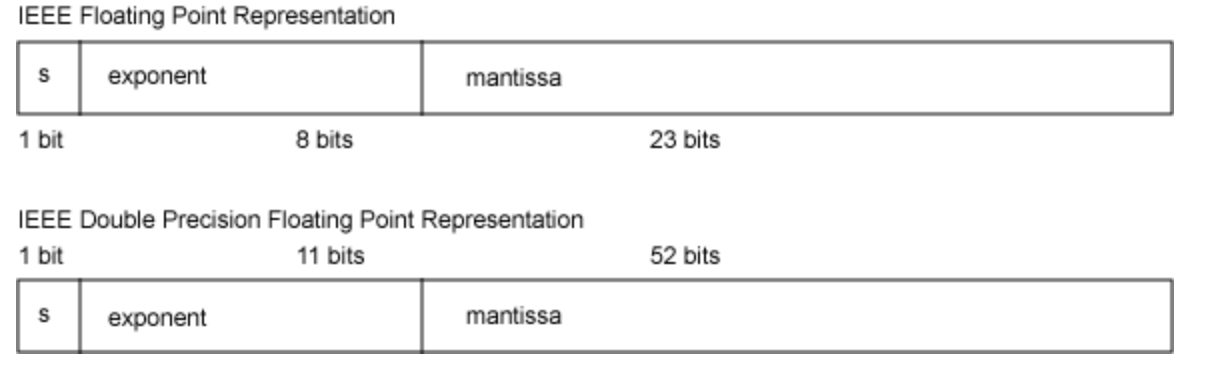
\includegraphics[width=0.7\textwidth]{floatingPoint_IEEE_layout.png}
\end{center}

\begin{tcolorbox}
	\textbf{Value of the IEEE-FloatingPoint number:} 
	\begin{center}
		$\color{blue}\mathbf{-1^{S} \times (1.0 + 0.M) \times B^{E-bias}}$ 
	\end{center}
	
 S = sign \\
 M = mantissa \\
 B = Basis $\in \mathbb{N}-\lbrace 1 \rbrace$ \\
 E = exponent  $\rightarrow $ Exponent range: $\lbrace e_{min}, ..., e_{max} \rbrace e_{min}, e_{max} \in \mathbb{Z}, e_{min} < e_{max}$ \\
 bias = 127 (single precision), 1023 (Double precision)
\end{tcolorbox}

\textbf{Largest machine number:} $x_{max} = \max|\M| = (1 - B^{-m}) \cdot  B^{e_{max}} $ \\
\textbf{Smallest machine number:} $x_{min} = \min|\M| = B^{-1} \cdot B^{e_{min}}$ \\

\underline{No suprise:} For modern computers $B = 2$ (binary system), the other parameters of universally implemented machine number system are:
\begin{itemize}
	\item single precision: $m=23, E \in \lbrace -125, ..., 128\rbrace \blacktriangleright$ 4 bytes 
	\item double precision: $m=52, E \in \lbrace -1021, ..., 1024 \rbrace \blacktriangleright $ 8 bytes 
\end{itemize}


% ------------
% Dense Matrices
\subsection{Dense Matrices}
\begin{tcolorbox}
	Dense(=generic) matrices store every entry in the matrix \textbf{(not many entries=0)}.  \vspace{-1mm}\\
	$\rightarrow$ All numerical libraries store the entries of a dense matrix $A /in \K^{m,n}$ in a \textbf{linear array of length $\color{red}\mathbf{mn}$ (or longer)}. 
\end{tcolorbox}

\textbf{Vectorisation options:} 
\begin{center}
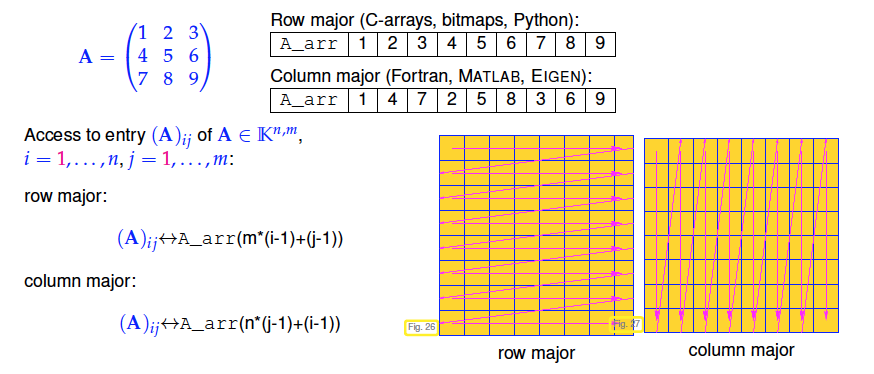
\includegraphics[width=0.8\textwidth]{DenseMatrix.png}
\end{center}

\textbf{$\rightarrow$ Remark:} Eigen Default: ColumnMajor

% ------------
% Sparse Matrices
\subsection{Sparse Matrices}
\begin{tcolorbox}
	“almost all” entries = 0 /“only a few percent of” entries $\not =$ 0"
\end{tcolorbox}




\subsubsection{Special storage formats for sparse matrices}
\textbf{- COO (Triplet/Coordinate format)} \\
Case: Sparse matrix $A \in \K^{m,n}$, this format stores triplets $(i, j, \alpha_{i,j}, 1\leq i \leq m, 1\leq j \leq n:$
\begin{center}
	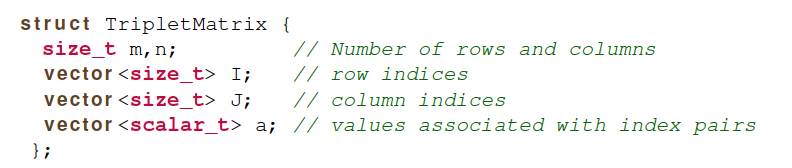
\includegraphics[width=0.8\textwidth]{SparseMatrix_COO.png}
\end{center}

All vectors have same size $\geq nnz(a)$, because repetitions of index pairs $(i,j)$ are allowed. \\

\textbf{- CRS (Compressed row storage)} \\
CRS format for a sparse matrix $A = (a_{ij}) \in \K^{n,n}$ keeps the data in three arrays:
\begin{center}
	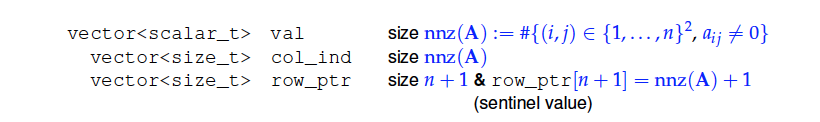
\includegraphics[width=0.9\textwidth]{SparseMatrix_CRS_structure.png}
\end{center}

Access to matrix entry $a_{ij} \not = 0,1 \leq i,j \leq n$:

\begin{center}
	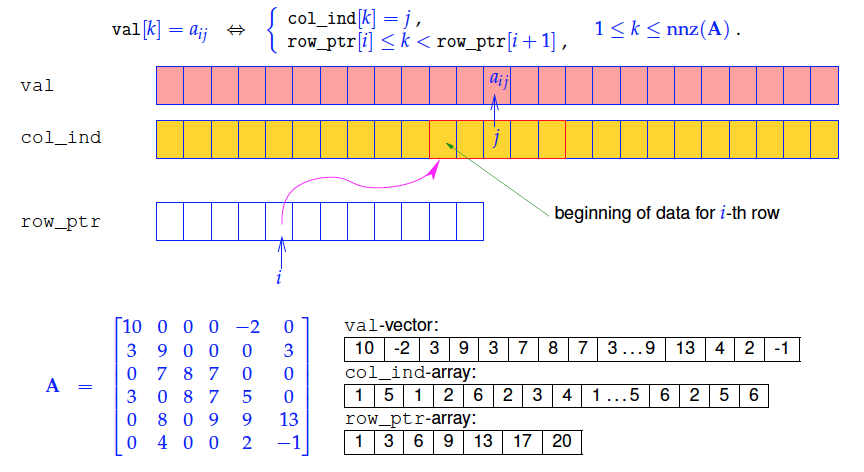
\includegraphics[width=0.9\textwidth]{SparseMatrix_CRS.png}
\end{center}

\textbf{Remark:} The CCS format is equivalent to the CRS format for the transposed matrix. \\



\subsection{Important Eigen Commands}

\subsubsection{Initializing Matrices, Vectors}

\textbf{Vector Creation \hspace{32mm} \color{blue}VectorXd (dynamic), VectorNd (fixed size)} \color{black}
\begin{lstlisting}[language=C++, caption=Initializing vectors]
	#include <Eigen/Dense>

	// Just allocate space for vector, no initialisation --> Exp: 20x1 vector
	VectorXd a(20);
	// Create vector with random entries of size nx1
	VectorXd b = VectorXd::Random( n , 1 )
	// Create row vector --> better: use of normal vector and transpose
	RowVectorXd c(10);
	
	
\end{lstlisting}



\textbf{Dense Matrix Creation \hspace{20mm} \color{blue}MatrixXd (dynamic), MatrixNd (fixed size)}

\begin{lstlisting}[language=C++, caption=Initializing dense matrices]
	#include <Eigen/Dense>
	#include <Eigen/Sparse>
	using namespace Eigen;
	
	// Just allocate space for matrix, no initialisation
	MatrixXd A(rows ,cols) ;
	// Zero matrix. Similar to matlab command zeros(rows, cols);
	MatrixXd B = MatrixXd::Zero(rows, cols);
	// Ones matrix. Similar to matlab command ones(rows, cols);
	MatrixXd C = MatrixXd::Ones(rows, cols);
	// Matrix with all entries same as value.
	MatrixXd D = MatrixXd::Constant (rows, cols, value);
	// Random matrix, entries uniformly distributed in [0,1]
	MatrixXd E = MatrixXd::Random(rows, cols);
	// (Generalized) identity matrix, 1 on main diagonal
	MatrixXd I = MatrixXd::Identity(rows , cols);
	// Matrix with only diagonal entries vom vector d_vector
	Eigen::MatrixXd D = d_vector.asDiagonal();
\end{lstlisting}

\textbf{Sparse Matrix Creation (CRS, and from Triplets(COO))}
\begin{lstlisting}[language=C++, caption=sparse matrix creation]
	#include <Eigen/Sparse>
	using namespace Eigen;
	
	// ----------------------------------
	// Creating CRS format Matrix
	SparseMatrix<double, Eigen::RowMajor> ExampleMatrix(rows, cols); 
	// ----------------------------------
	// Creating Matrix from Triplets
	// Definition of a SparseMatrix
	SparseMatrix<double> C(n,m);

	// TripletList to save some triplets (COO format)
	std::vector<Triplet<double>> tripletList;
	// Triplet entry
	Triplet<double> triplet (i, j, value); 	 
	// Saving Triplet in TripletList
	tripletList.push_back(triplet);
	//Fill Sparse Matrix with triplets in tripletList
	C.setFromTriplets(tripletList.begin(), tripletList.end());
	//Compress Sparse Matrix
	C.makeCompressed();
\end{lstlisting}



\subsubsection{Matrix/Vector Access}
\begin{lstlisting}[language=C++, caption=matrix manipulation]
	
	// Get col, row size of matrix & number of elements
	int cols = A.cols();
	int rows = A.rows();
	std::cout << "It has " << m.size() << " coefficients" << std::endl;
	
	// Get size of vector m (nr. of elements = size)
	int elements = m.size()
		
	// Get entry of matrix --> Example A(2,3) value
	int entryValue = A(2,3);
	
	// Get i'th row, column from matrix A
	std::cout << A.col(J)  << std::endl;
	std::cout << A.row(i) << std::endl;
	
	// Block containing the first q rows (matrix)
	std::cout << matrix.topRows(q) << std::endl;
	
	// Block containing the first n elements (vector)
	std::cout <<	vector.head(n)	<< std::endl;
	
	// Get block(submatrix) --> Block starting from (0,0) with dimension ixi
	std::cout << M.block(0,0,i,i) << std::endl;
\end{lstlisting}


\subsubsection{Matrix Reshapening}
...

\subsubsection{Operations}
...

\subsubsection{Runtime plotting with FigureClass}
...

\subsubsection{Solvers for LSE in Eigen }
	\begin{lstlisting}[language=C++, caption=LSE solvers]
	
	// Gaussian elimination with partial pivoting, Code 2.3.41
	x = A. lu().solve(b); // lu() is short for partialPivLu()
	
	// Gaussian elimination with total pivoting
	x = A. fullPivLu().solve(b); // total pivoting
	
	// An elimination solver based on Householder transformations		
	Eigen::HouseholderQR<MatrixXd> solver(A);
	x = solver.solve(b) ;	
	
	// Use singular value decomposition (SVD)	
	x = A.jacobiSvd(Eigen::ComputeThinU | Eigen::ComputeThinV).solve(b);	
		
	\end{lstlisting}


\subsubsection{Solvers for sparse LSE}
	\begin{lstlisting}[language=C++, caption=LSE solvers (sparse)]
		Eigen::SparseLU<SparseMatrix> solver(A) ;
		x = solver.solve(b) ;
	\end{lstlisting}

\begin{tcolorbox}
	When solving linear systems of equations directly dedicated sparse elimination \textbf{solvers from numerical libraries} have to be used! \\
	
	$\rightarrow$ System matrices are passed to these algorithms in sparse storage formats to convey information about zero entries.	
\end{tcolorbox}





% -------------------------------------------------------------
% Machine Arithmetic
% -------------------------------------------------------------
\newpage
\section{Machine Arithmetic}

$\rightarrow$ Computers cannot compute “properly” in $\R$: \\
(numerical computations may not respect the laws of analysis and linear algebra)\newline

$\M \subset \R$ is the set of \textbf{machine numbers} (finite, discrete) \\
$\rightarrow$ not closed under elementary arithmetic operations! \\

\begin{tabular}{lll}
	$op$: 	& 		$\R \times \R \rightarrow \R$ & 			$op \in \lbrace +, -, *, / \rbrace$	\\
			& 		$\M \times \M \not\rightarrow \M$  											\\
																								\\
	$\widetilde{op}$: &  		$\M \times \M \rightarrow \M$ 	& $\Rightarrow$ $\widetilde{op} = rd \circ op \quad $ (on computers) 
\end{tabular}

\begin{center}
	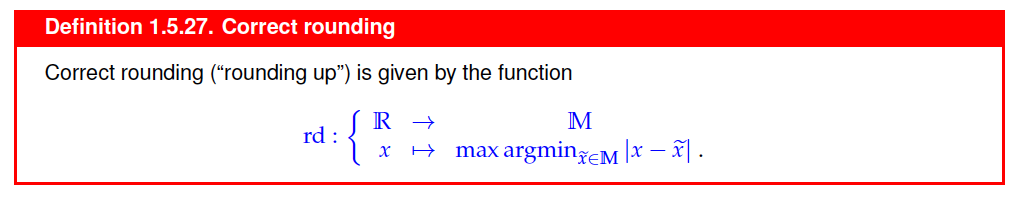
\includegraphics[width=1.0\textwidth]{rounding_function.png}
\end{center}

\begin{tcolorbox}
\hspace{3mm}	
	For $\star \in \lbrace +, -, *, / \rbrace$: \quad $x \widetilde{\star} y = rd(x \star y)$  \quad \textit{where rd(...) is the rounding function} 
\hspace{3mm}	
\end{tcolorbox}
\hspace{3mm}	

% ----------------------
% Controlling roundoff error	
\subsection{Controlling roundoff error}	
\textbf{EPS} (largest relative error) := $\max\limits_{x \in I\setminus \lbrace 0 \rbrace} \frac{|rd(x) - x|}{|x|}$ \quad \textit{where $I = \lbrack \min |\M|, \max |\M| \rbrack$}
\\

... can also be computed by the defining parameters B (base) and m (length of mantissa): \\
\begin{equation*}
		EPS = \frac{1}{2} B^{1-m}
\end{equation*}
		
\begin{center}
	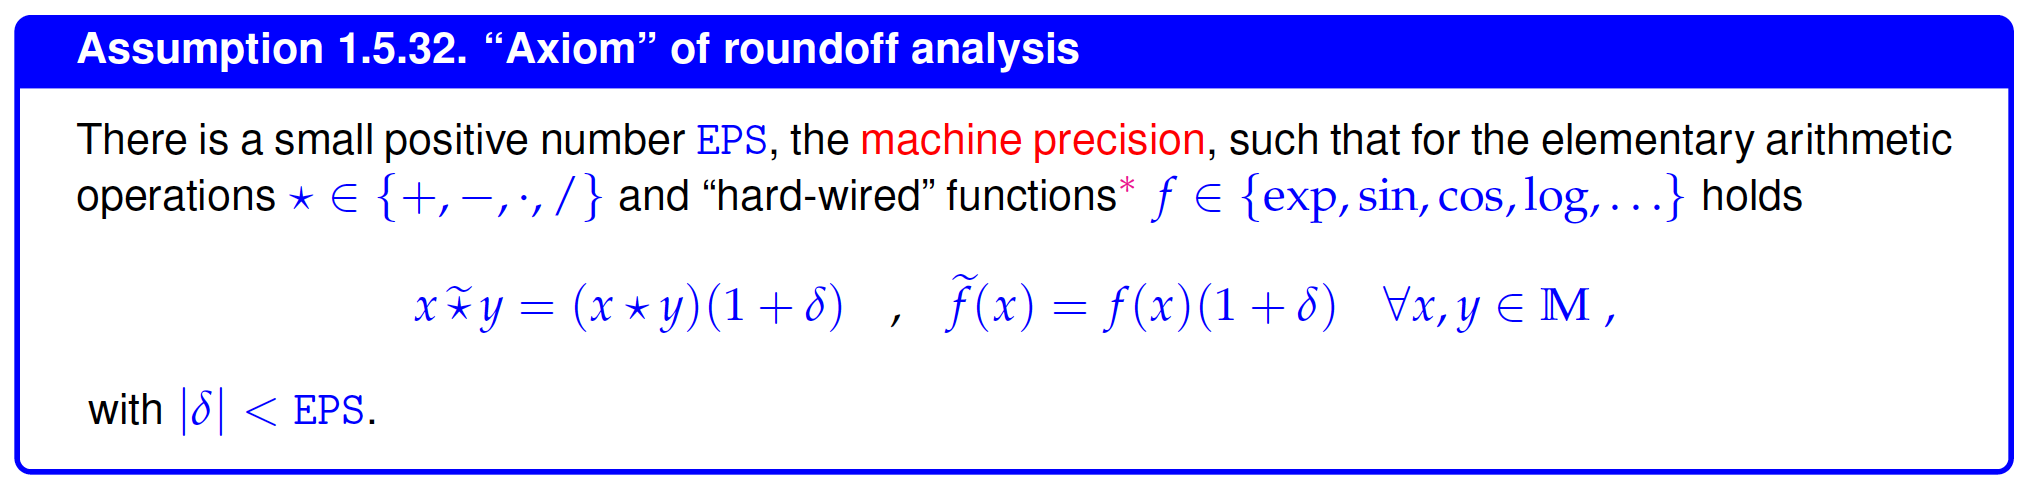
\includegraphics[width=1.0\textwidth]{axiom_roundoff_analysis.png}
\end{center}
	
\subsubsection{Getting machine precision with c++}
\begin{lstlisting}[language=C++]
	#include <iostream>
	#include <limits> 	// get various properties of arithmetic types
	int main() {
		std::cout.precision(15); 	// set floating point precision
		std::cout << std::numeric_limits<double>::epsilon() << std::endl;
	}
\end{lstlisting}

\textbf{Output:} \quad $2.22044604925031e^{-16}$ \\
\pagebreak

\subsubsection{Experiment - Adding EPS to 1}
\begin{lstlisting}[language=C++]
	cout.precision(25);
	double eps = numeric_limits<double>::epsilon();
	cout << fixed << 1.0 + 0.5*eps << endl
			<< 1.0 - 0.5*eps	<< endl
			<< (1.0 + 2/eps) - 2/eps << endl;			// cancellation here
\end{lstlisting}

\textbf{Output:} 

\begin{lstlisting}[language=c++]
1.000000000000000000000000
0.9999999999999998889776975
0.0000000000000000000000000
\end{lstlisting}


\hspace{5mm}	
\subsubsection{Testing equality with zero $|$ x == 0.0} 
\textbf{Numerical crime} for result of floating point computations \\
$\rightarrow$ Replace with test of relative smallness! \\
	
	... example of testing with relative smallness ...
	
\hspace{6mm}

	
% -----------
% Cancellation 
\subsection{Cancellation}
 

 \begin{minipage}{0.6\textwidth}
 	... = \textbf{subtraction of almost equal numbers} \\
 $\blacktriangleright$ extreme ampilifcation of relative errors \\
 $\blacktriangleright$ if inevitable, substraction prone to cancellation should be done as early as possible
 \end{minipage}
\hfill
 \begin{minipage}{0.3\textwidth}\raggedleft
 		 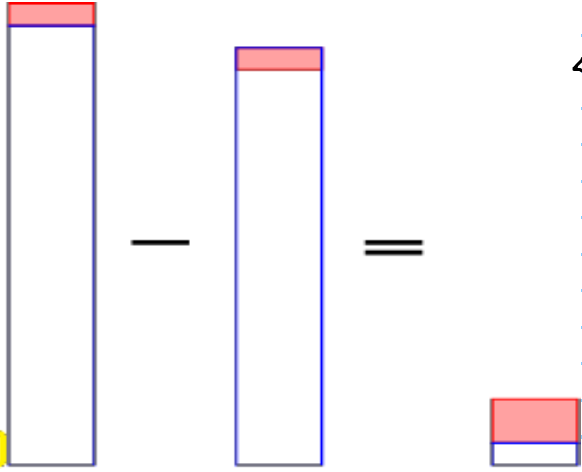
\includegraphics[width=0.8\textwidth]{cancellation_illustration.png}
 \end{minipage}


\hspace{5mm}
\subsubsection{Example  1 - Cancellation when evaluating difference quotients}
\begin{equation*}
	f'(x) \approx \frac{f(x+h) - f(x)}{h} \quad \quad , |h|<<1	
\end{equation*}
\hspace{10mm}
$\Rightarrow$ Cancellation will happen here: $f(x+h) - f(x)$


\subsubsection{Example  2 - Cancellation in Gram-Schmidt orthogonalisation}

\begin{minipage}{0.6\textwidth}
Cancellation when computing orthogonal projection of vector a onto space spanned by vector b.
\begin{equation*}
	p = a - \frac{a \cdot b }{b \cdot b}b
\end{equation*}
If a, b are nearly parallel: $p \approx 0$ $\rightarrow$ Cancellation
\end{minipage}
\begin{minipage}{0.3\textwidth}\raggedleft
 		 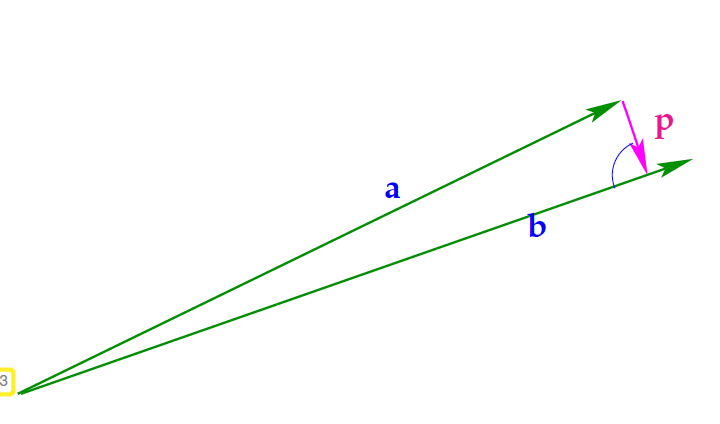
\includegraphics[width=1.0\textwidth]{cancellation_gramSchmidt.png}
 \end{minipage}



\subsubsection{Tricks to avoid cancellation}
 
 \begin{tcolorbox}
 \textbf{USE OF ALTERNATIVE FORMULAS:}
 \begin{itemize}
  \item Use mathmatic identities (trigonometric, definitions, ...)
  \item Approximation with Taylor Series $\rightarrow$ Choosing m large enough
  \item Sometimes: Use of case distinctions
\end{itemize}
\end{tcolorbox}


% ----------------
% Numerical stability
\subsection{Numerical stability}

\subsubsection{Problem description}
\begin{minipage}{0.6\textwidth}
	\begin{equation*}
	F: X \subset \R^{n} \longrightarrow Y \subset \R^{m}	
	\end{equation*}
	\begin{center}
		(X := data space and Y := result space)
	\end{center}
\end{minipage}
\begin{minipage}{0.3\textwidth}\raggedleft
	\begin{center}
	 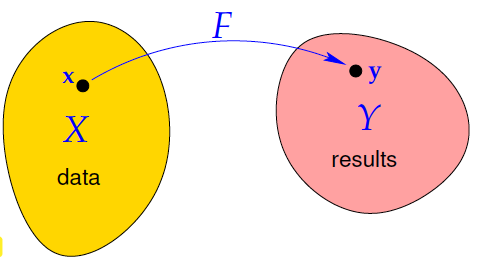
\includegraphics[width=1.0\textwidth]{stable_problem_desc.png}
\end{center}
\end{minipage}


\subsubsection{Numerical algorithm}
\begin{itemize}
	\item Problem: \quad  \quad $F: X \subset \R^{n} \longrightarrow Y \subset \R^{m}	$
	\item Algorithm: \quad  $\tilde{F}: X \rightarrow \tilde{Y} \subset \M$
\end{itemize}



\subsubsection{Stable Algorithm (= Good Algorithm)}
\begin{center}
	 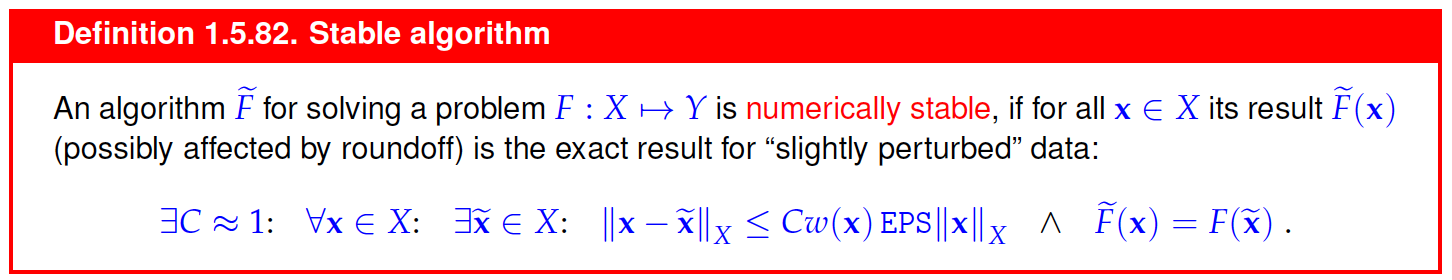
\includegraphics[width=1.0\textwidth]{stable_algorithm1.png}
\end{center}

\begin{center}
	 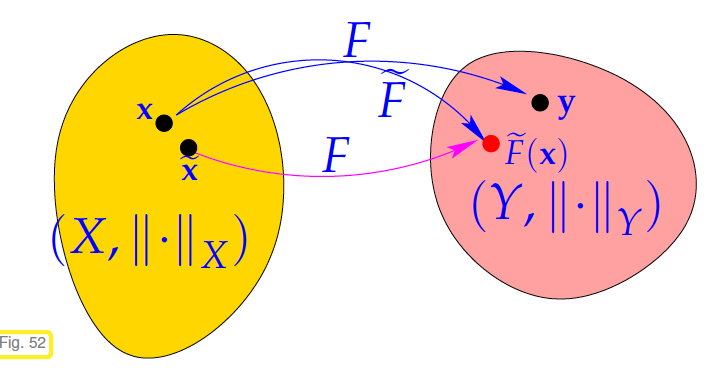
\includegraphics[width=0.6\textwidth]{stable_algorithm2.png}
\end{center}

% -------------------------------------------------------------
% Linear systems of equations
% -------------------------------------------------------------
\newpage
\section{Linear Systems of Equations}

\subsection{Existence and Uniqueness of solutions}
...

\subsection{Sensitivity of Linear Systems}

The Sensitivity of a problem (for given data) gauges the impact of small perturbations of the data on the result. \\

\begin{tcolorbox}
		\vspace{-5mm}
	\begin{equation*}
	\textbf{Condition Number of a Matrix } A \in \R^{n,n}:\quad \text{cond}(A) := ||A^{-1}||\cdot||A||
	\end{equation*}
\end{tcolorbox}

\begin{center}
		\textbf{small} changes of data $\Rightarrow$ \textbf{large} perturbation of result $\Rightarrow$ \textbf{ill}-conditioned problem $\Rightarrow$ $\text{cond}(A) >> 1$ $\Rightarrow$ columns/rows of $A$ are almost linearly dependent \\
\end{center}

\textbf{Remark:} If $cond(A) \gg 1$, a stable algorithm can produce solutions with large rel. error!


\subsection{LSE with low-rank perturbation}

\begin{tcolorbox}
Adding a tensor product of two vectors to a matrix := \textbf{rank-1 modification}	
\end{tcolorbox}

Given $A \in \K^{n,n} \mapsto \mathbf{\color{blue}\tilde{A} := A + uv^H}$ we can use the \textbf{Sherman-Morrison-Woodburry formula} to solve $\tilde{A}\tilde{x} = b$ more efficiently provided that the LU-decomposition of $A$ is already known.

\begin{equation*}
	\tilde{x} = \textcolor{orange}{A^{-1}b}-\frac{\textcolor{red}{A^{-1}u}(v^H(\textcolor{orange}{A^{-1}b}))}{1+v^H(\textcolor{red}{A^{-1}u})}
\end{equation*}

Note that $\textcolor{orange}{A^{-1}b}$ und $\textcolor{red}{A^{-1}u}$ can be computed more efficiently using the LU-decomposition of $A$. The resulting complexity is $O(n^2)$.

\subsection{LU-Factorization of sparse Matrices}

\begin{center}
	$A$ sparse $\not\Rightarrow$ LU-factors sparse
\end{center}

A \textbf{fill-in} at position $(i,j)$ of the decomposition $A=LU$ occurs if $a_{ij} = 0$ but $u_{ij} \neq 0$ or $l_{ij} \neq 0$.

\subsubsection{Using LU factorization to solve a LSE}
Solving a $n \times n$ linear system of equations by LU factorization:
\begin{enumerate}
	\item LU decomposition: \hspace{8mm} $A=LU$ \hspace{3mm} $\rightarrow O(n^3)$
	\item Forward substitution: \hspace{4mm} $Lz=b$ \hspace{5mm} $\rightarrow O(n^2)$
	\item Backward substitution: \hspace{2mm} $Ux=z$ \hspace{3mm} $\rightarrow O(n^2)$
\end{enumerate}


\subsubsection{Arrow Matrices}

The LU-decomposition of an arrow matrix pointing into the upper left corner leads to massive fill-in, one that points to the bottom right corner doesn't, however. Thus, it's easier to transform one into the other via a permutation matrix. The resulting decomposition without pivoting requires only $O(n)$.

\begin{center}
	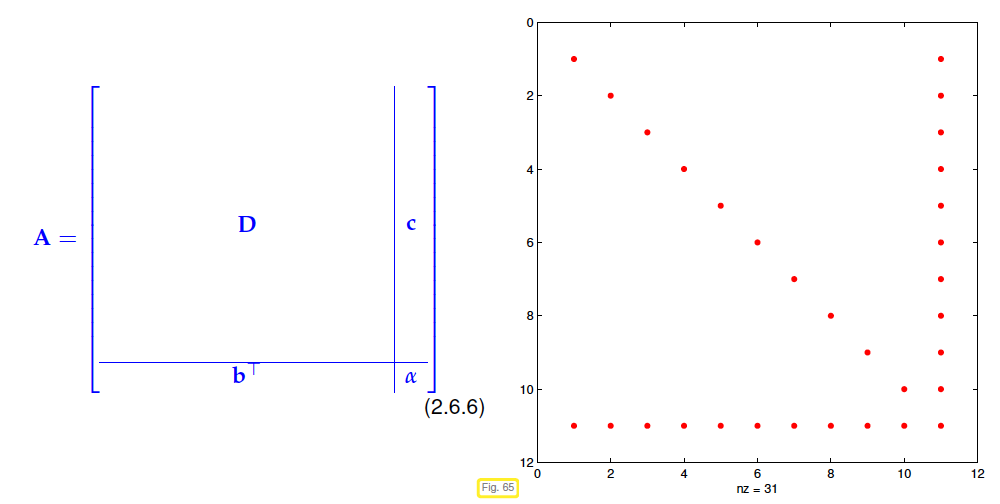
\includegraphics[width=0.7\textwidth]{arrow_matrix.png}
\end{center}

\begin{tcolorbox}
	\vspace{1mm}
	\textbf{Remark for solving LSE with arrow matrix:}
	\begin{center}
		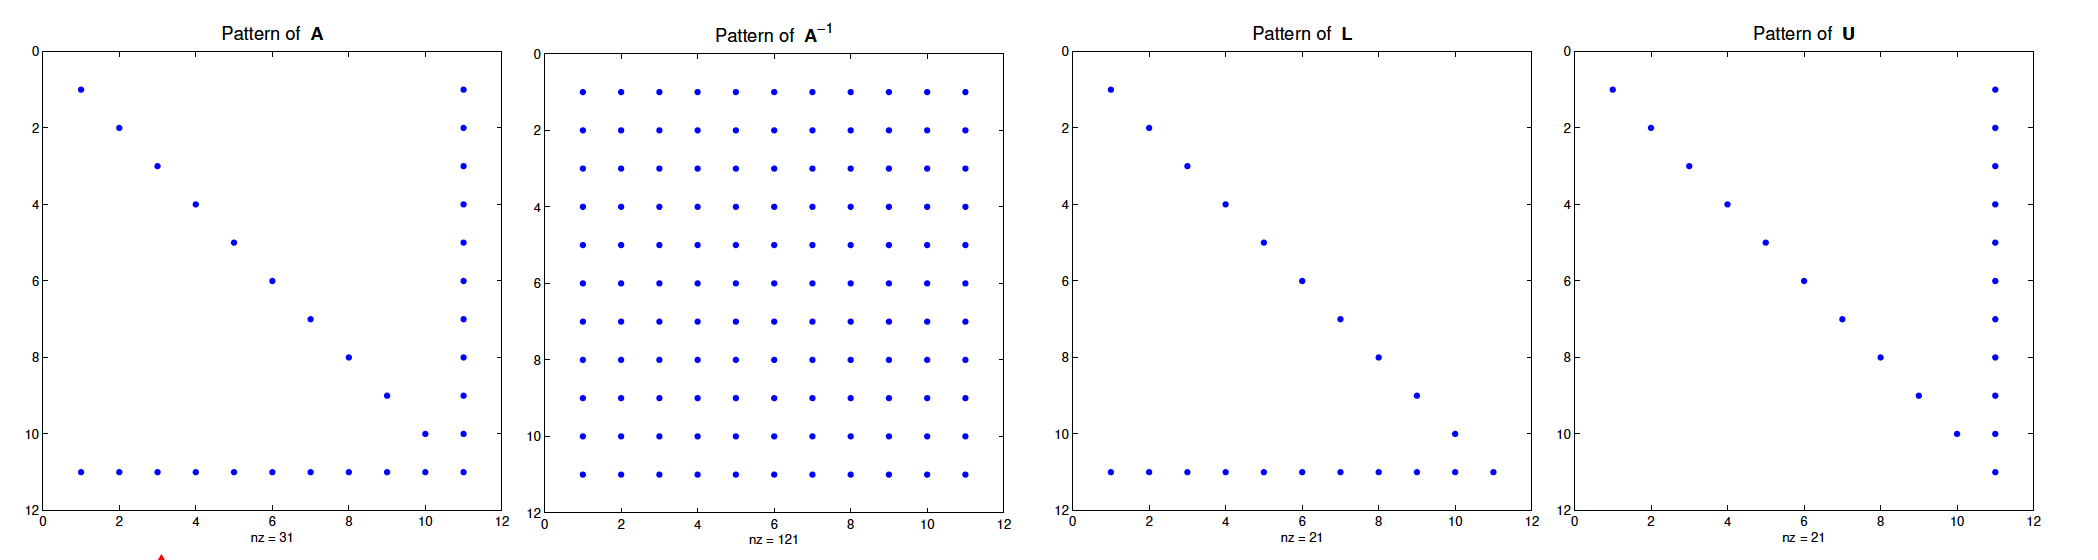
\includegraphics[width=0.8\textwidth]{arrow_matrix_inverse.png} \\
		$\rightarrow$ A, L, U are sparse \quad \quad \textbf{BUT:} $A^{-1}$ is not sparse! \\
	\end{center}

	Besides stability and efficiency issues, this is another reason why using \color{red} \\
	$x = A.inverse()*y$ \color{black} instead of \color{blue}$\mathbf{y=A.lu().solve(b)}$ \color{black} is usually a major blunder. 
\end{tcolorbox}


\subsubsection{Banded Matrices}

\begin{center}
	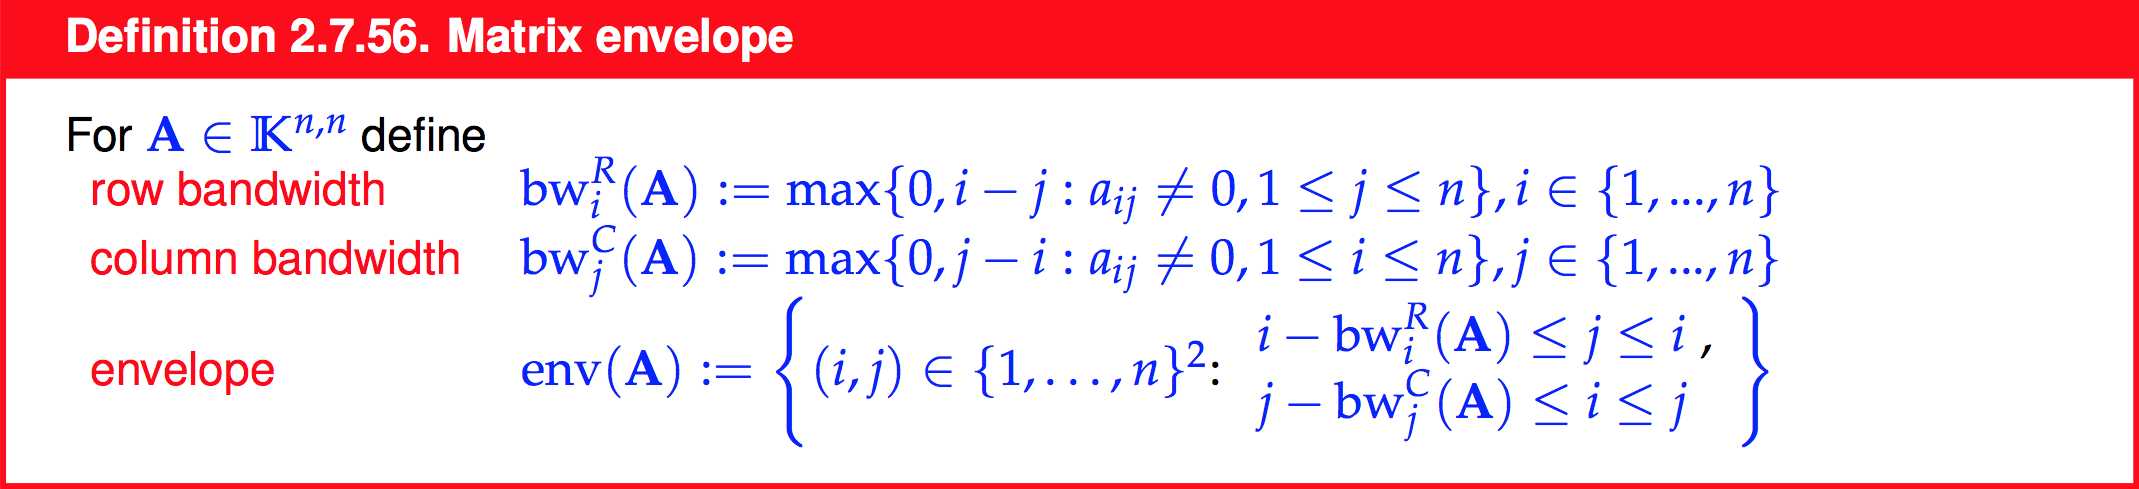
\includegraphics[width=350pt]{envelope}
\end{center}

For the LU-decomposition of the regular matrix $A \in \K^{n,n}$ the \textbf{fill-in is confined} to $\text{env}(A)$.

\begin{center}
	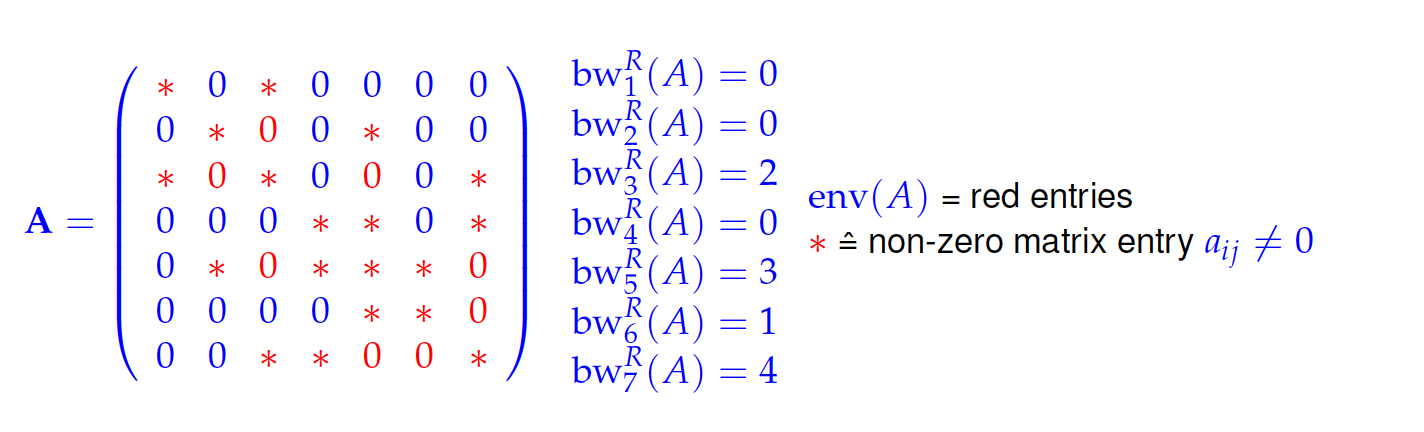
\includegraphics[width=350pt]{envelope2.png}
\end{center}

\subsubsection{Structurally Symmetric Matrix}

\begin{center}
	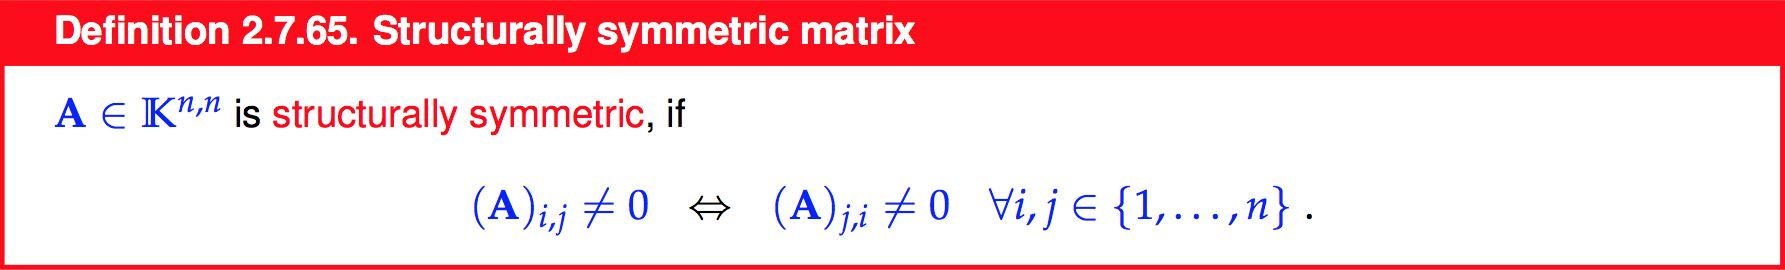
\includegraphics[width=310pt]{ssmatrix.png}
	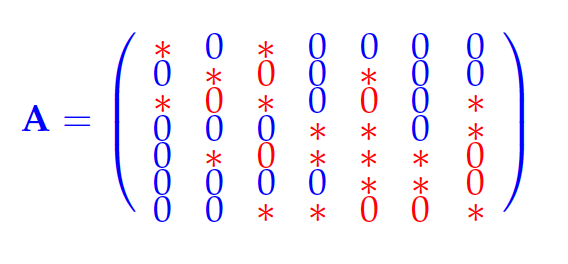
\includegraphics[width=0.24\textwidth]{strucSymMatrix.png}
\end{center}

\subsection{Stable Gaussian Elimination Without Pivoting}

Recall the following insights:
\begin{itemize}[noitemsep]
	\item Special structure of a matrix avoids fill-in during Gaussian Elimination/LU-decomposition without pivoting
	\item Pivoting can lead to massive fill-in
	\item Fill-in reducing effect of reordering can be cancelled out by subsequent row swapping in the course of pivoting 
\end{itemize}

\textbf{However}, \textbf{pivoting is necessary} to provide a numerically stable Gaussian Elimination/LU-decomposition. \\

For certain classes of matrices, however, pivoting isn't required to for a stable elimination:

\begin{description}[labelindent=16pt,style=multiline,leftmargin=7cm, noitemsep]
	\item[Diagonally Dominant Matrix:] The absolute value of the components in the diagonal are larger than the sum of the absolute values of their respective row. $\sum_{j\neq k}|a_{jk}| \leq |a_{kk}|$
	\item[s.p.d. Matrix:] Symmetric/Hermitian positive definite matrices
\end{description}


\subsection{Cholesky Decomposition}
... (see chapter 2.8.13)

% -------------------------------------------------------------
% Direct Methods for Linear Least Squares Problems
% -------------------------------------------------------------
\newpage
\section{Direct Methods for Linear Least Squares Problems}

\begin{tabular}{lll}
$A \in R^{m,n}$ dense and n small		& $\rightarrow$ &   Use \textbf{orthogonal transformations methods}  \\ 
															&  & ($\rightarrow$ GramSchmidt is numerically \color{red}{not stable}\color{black}) \\
															&	& - Householder Reflection \\
															&  & - Givens Rotation \hspace{5mm}\\
$A \in R^{m,n}$ sparse and m,n big 	& $\rightarrow$ &	 Use \textbf{normal equations in the expanded form}   \\ 

\end{tabular}


\subsection{General - Least Squares}

\textbf{Problem:}  \quad Overdetermined linear systems of equations (see below)
\begin{center}
	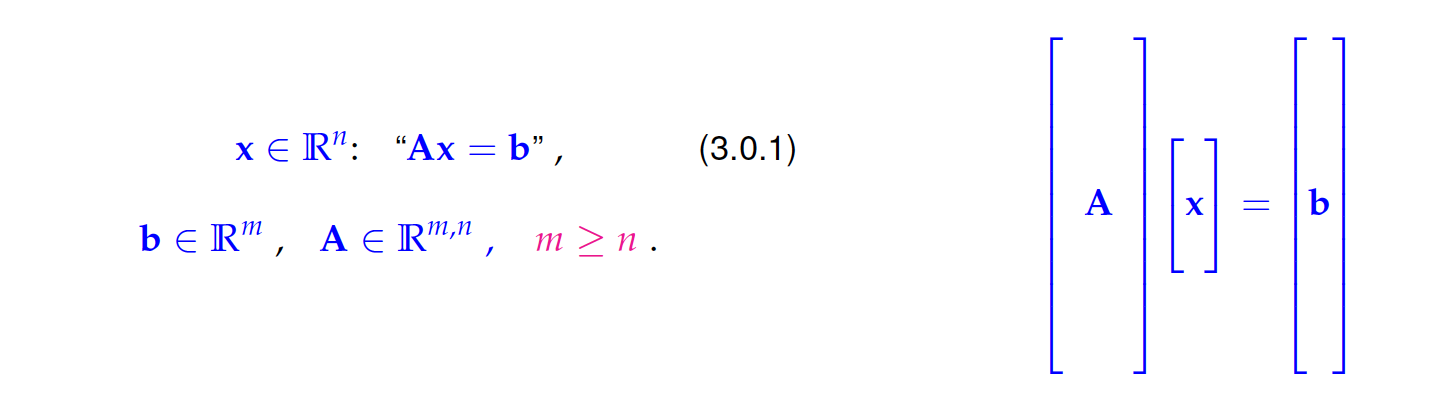
\includegraphics[width=350pt]{leastsquares_overview.png}
\end{center}


The system $Ax=b$ has a solution, if and only if the right hand side vector b lies in the image (range space) of the matrix $A$:
\[
	\exists x \in \R^{n}: \quad Ax = b \Leftrightarrow b \in \mathcal{R}(A)
\]


\rule{40pt}{1pt} \\
ERWEITERN!
\begin{center}
	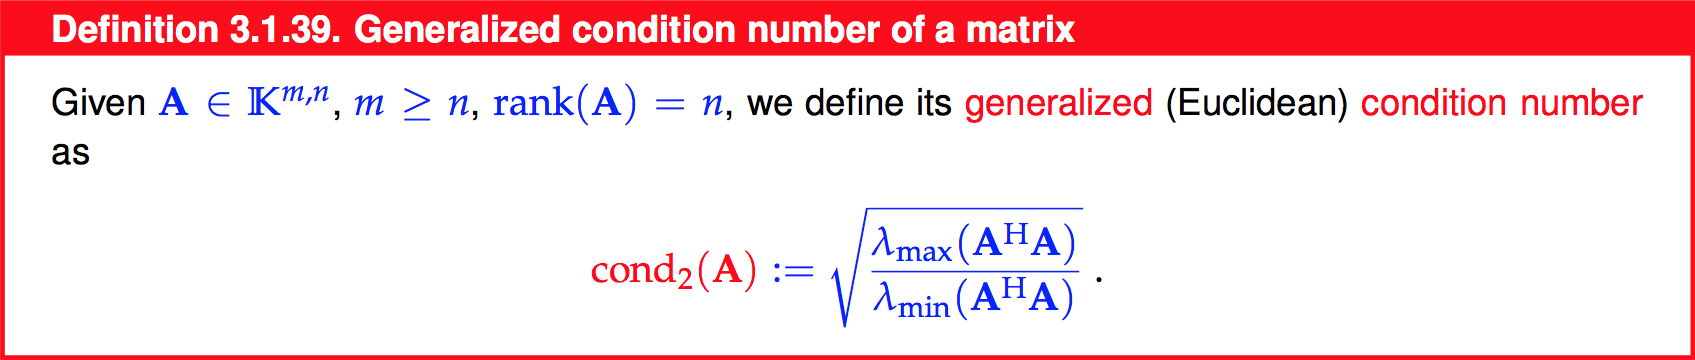
\includegraphics[width=350pt]{cond.png}
\end{center}

This definition agrees with the previous definition in case $A$ is regular. \\
\rule{40pt}{1pt}



\subsection{Least squares solution concept}

\textbf{Idea:} \quad We seek x that makes the residual $r:=b-Ax$ small.
\begin{center}
	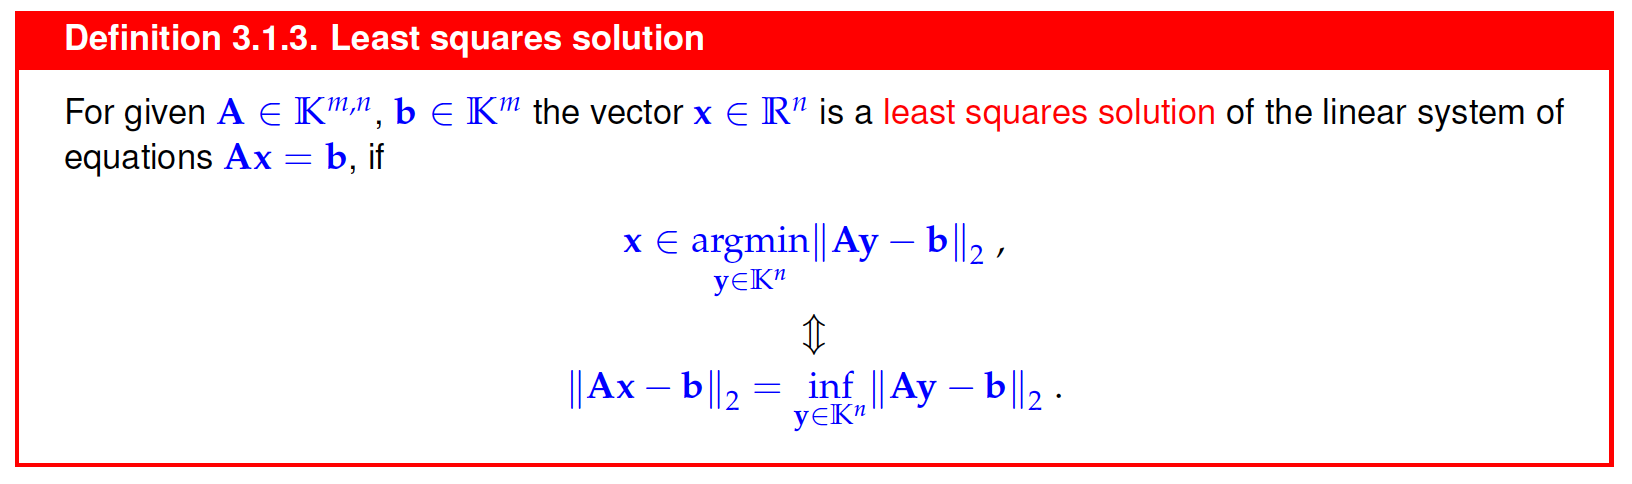
\includegraphics[width=350pt]{leastsquares_solution.png}
\end{center}

$\rightarrow$ But they are different situations and different methods to get this $x$!


\subsection{Normal Equation Method}

\subsubsection{Standard Method}

\begin{tcolorbox}
\textbf{Given:}\\
$Ax = b$ (overdetermined linear system of equations) \\
$m \geq n$, $rank(A)=n$ ,  $b \in \R^{m}$\vspace{2mm}\\
\textbf{Task:} \vspace{-2mm}
\begin{enumerate}[noitemsep]
	\item Compute regular matrix $C := A^TA \in \R^{n,n}$
	\item Compute right hand side vector $c := A^Tb$
	\item Solve linear system of equation $Cx = c$
\end{enumerate}
\end{tcolorbox}

\textbf{- Normal equation definition:}
\begin{center}
	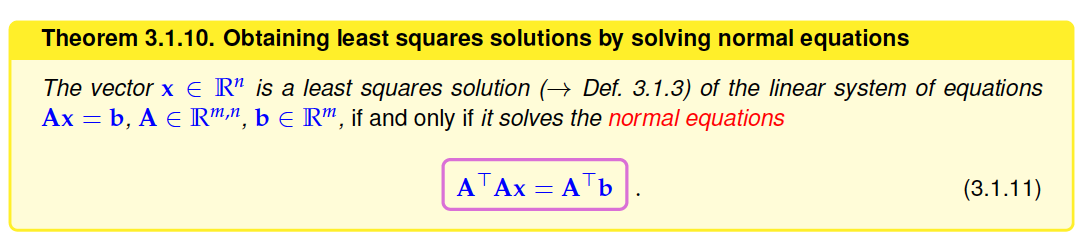
\includegraphics[width=380pt]{normalEquationDef.png}
\end{center}

\textbf{- Uniqueness of Least square solutions:}
\begin{center}
	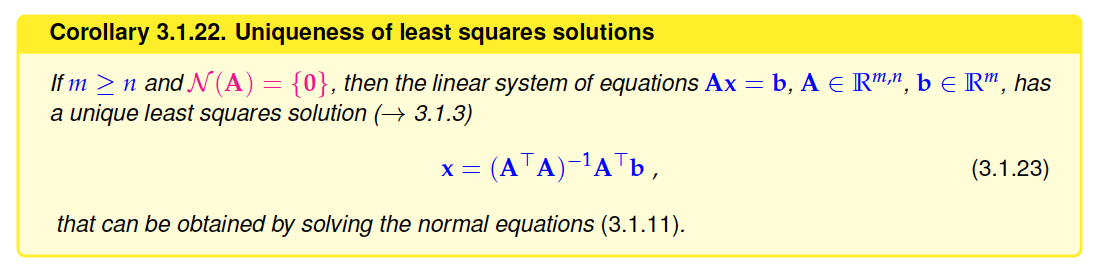
\includegraphics[width=380pt]{normalEquationUniqueness.png}
\end{center}


$\rightarrow A^TA$ is \color{blue}s.p.d. (symmetric positive definite) \color{black} if $\mathcal{N}(A) = \lbrace 0 \rbrace$ \\

\textbf{Remark: Full Rank condition (FRC)} \\
For a matrix $A \in \R^{m,n}$ with $m \geq n$ is equivalent: \quad $\mathcal{N}(A) = \lbrace 0 \rbrace \Leftrightarrow rank(A)=n$ \\

\begin{tcolorbox}
\color{red}\textbf{Problem 1:} Normal equations are numerically problematic! \\

\[ 
	A = 
	\begin{bmatrix}
	1 & 1 \\ 
	\delta & 0 \\
	0 & \delta	
	\end{bmatrix}
	\quad
	\Rightarrow
	\quad
	A^TA = 
	\begin{bmatrix}
	1 + \delta^2 & 1 \\
	1 & 1 + \delta^2 	
	\end{bmatrix}
\] 
If $\delta \approx \sqrt{EPS}$, then $1 + \delta^2 = 1$ in $\M$. Hence the computed $A^TA$ will fail to be regular, though $rank(A) = 2, cond_2(A) \approx \sqrt{EPS}$! \hspace{3mm}\\

\textbf{Problem 2:} Loss of sparsity! \\
$A$ sparse $\not \Rightarrow A^TA$  sparse!
\end{tcolorbox}



\subsubsection{Extended Method}

The extended method, compared to the standard one, \textbf{preserves sparsity}. However, the conditioning of the systems does not change. It also \textbf{doesn't require the computation of} $\mathbf{A^HA}$. \\

The problem can be solved using the residual defined as $r := Ax - b$:

\begin{equation*}
	B\begin{bmatrix}r \\ x \end{bmatrix} := \begin{bmatrix}
		-I & A \\ A^H & 0
	\end{bmatrix} \begin{bmatrix}
		r \\ x
	\end{bmatrix} = \begin{bmatrix}
		b \\ 0
	\end{bmatrix}
\end{equation*}

\subsection{Orthogonal Transformation method}
\begin{tcolorbox}
	\textbf{Idea:} Conversion of the LSE $Ax=b$ by row transformations to an equivalent LSE $Ux=\tilde b$ ,which is easier to solve because it has a triangular form. \vspace{2mm}\\
$\Rightarrow$ Transform $Ax=b \longrightarrow \tilde Ax = \tilde b$ such that $Lsq(A,b) = Lsq(\tilde A, \tilde b)$ \\

\textbf{Result:} Triangular least squares problem, which is easier to solve:
\begin{center}
	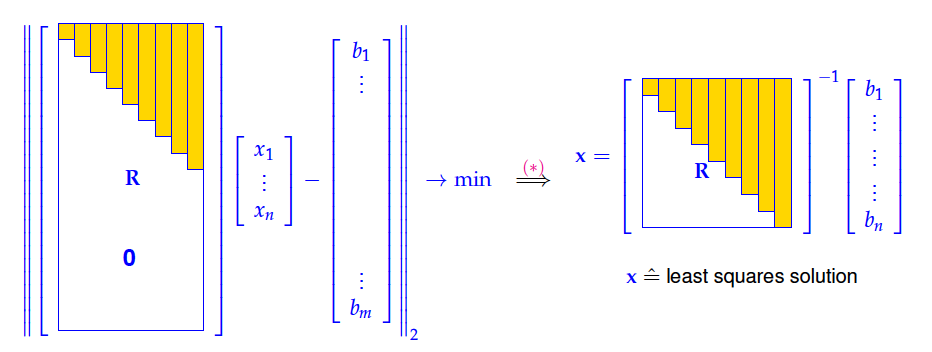
\includegraphics[width=380pt]{orthogonalTransformation_1.png}
\end{center}

\textbf{Solution:} \quad $x=R^{-1}(b)_{1:n}$ \hspace{35mm} R is regular, if $rank(A)=n$
\end{tcolorbox}

\vspace{10mm}


Generally, we're looking for two matrices $Q$ and $R$, such that
\begin{equation*}
	A = QR
\end{equation*}
This is possible to achieve using the \textbf{Gram Schmidt Orthonormalization}. This procedure isn't numerically stable. \\

ERGAENZEN VON ECONOMICAL and FULL QR DECOMPOSITION

\subsubsection{Householder Reflections}

\begin{tcolorbox}
\begin{equation*}
	Q = H(v) := I - 2\frac{vv^H}{v^Hv}\text{ mit } v = \frac{1}{2}(a \pm ||a||_2 e_1)
\end{equation*}
\end{tcolorbox}

TODO: Hinweis Cancellation und daherige Fallunterscheidung! Und bildliche Interpretation!

\subsubsection{Givens Rotation}

Alternatively, the Givens Rotation can be used instead of the Householder Reflections. \\

$\Rightarrow$ QR-Decomposition by Givens preserves bandwith of banded matrices.
 
\subsection{Singular Value Decomposition (SVD)}




%--------------------------------
\subsection{Total Least Squares}
We have generally considered overdetermined linear systems of equations $Ax = b$, for which only the right handside vector b was affected by measurement errors. But it is also possible that A and b are perturbed (affected by measurements errors)!

\begin{tcolorbox}
\textbf{Given:}\\
$Ax = b$ (overdetermined linear system of equations) \\
$m \geq n$, $rank(A)=n$ ,  $b \in \R^{m}$\vspace{2mm}\\
\textbf{Known:}  \\
LSE would be solvable if A, b were not perturbed  \vspace{2mm}\\
\textbf{Task:} \\
Find the nearest solvable LSE \\
$\rightarrow  \hat A \in \R^{m,n}$ ,  $\hat b \in \R^{m}$ with: \\
\[ \lVert \lbrack A \text{ }b \rbrack - \lbrack \hat A \text{ } \hat b \rbrack\rVert_{F} \rightarrow min, \quad \hat b \in \mathcal{R}(\hat A) \] 
\end{tcolorbox}


$\Rightarrow \lbrack \hat A \text{ } \hat b \rbrack \in \R^{m, n+1}$ \textbf{is the rank-n best approximation of}  $\lbrack A \text{ }b \rbrack$ \\

\textbf{Calculation:} \\
(1) SVD of $\lbrack A \text{ }b \rbrack = U \Sigma V^{T}$, \quad \quad $V \in \R^{n+1, n+1}$ \\
\[ \lbrack A \text{ }b \rbrack =  U \Sigma V^{T} = \sum_{j=1}^{n+1} \sigma_j (U)_{:,j} (V)_{:,j}^{T} \quad \Rightarrow \quad  \lbrack \hat A \text{ } \hat b \rbrack = \color{red}\sum_{j=1}^{n} \color{black}\sigma_j (U)_{:,j} (V)_{:,j}^{T} \]
\begin{center}
$\Rightarrow \hat A = (\lbrack \hat A \text{ } \hat b \rbrack )_{1:n, 1:n}$, \quad $\hat b = (\lbrack \hat A \text{ } \hat b \rbrack )_{1:n, n+1}$ \vspace{2mm}\\
	Due to orthogonality: $\lbrack \hat A \text{ } \hat b \rbrack (V)_{:n+1} = 0$
	\vspace{10mm}\\

	$x = \hat A^{-1} \hat b =\color{red} ... (correct formula)...$
 
\end{center}


%--------------------------------
\subsection{Constrained Least Squares}

!! Some data are considered accurate $\rightarrow$ mix interpolation and least squares fitting

\begin{tcolorbox}
\textbf{Linear least squares problem with linear constraint:}
\vspace{2mm} \\
Given: \\
$A \in \R^{m,n}, m \geq n, rank(A) = n, b \in \R^{m}$\\
 $C \in \R^{p,n}, m < n, rank(C) = p, d \in \R^{p}$ \\

Find: \\
$x \in \R^{n}$ with $ \lVert Ax - b\rVert_{2} \rightarrow min $, \quad \quad $Cx =d$ (linear constraint)	
\end{tcolorbox}

\subsubsection{Solution with normal equations (and Lagrange parameter)}

\textbf{Idea:} coupling the constraint using the Lagrange multiplier $m \in R^{p}$

\begin{equation*}
	x = \argmin_{x \in \R^{n}}  \max_{m \in \R^{p}} L(x,m)  \quad \longrightarrow \quad L(x,m) ) := \frac{1}{2} \lVert Ax - b\rVert^{2} + m^{T} (Cx - d)
\end{equation*}

Simple heuristics behind Lagrange multipliers: $\max_{m \in \R^{p}} L(x,m) = \infty $ in case of: $Cx \not = d$

\begin{equation*}
	\text{Augmented normal equation: \quad}
  	\begin{bmatrix}
  		A^{T}A 	& C^{T} \\
  		C 			& 0 
  	\end{bmatrix}
  	\begin{bmatrix}
  		x \\
  		m
  	\end{bmatrix} 
  	=
  	\begin{bmatrix}
  		A^{T}b \\
  		d
  	\end{bmatrix} 
\end{equation*}

\subsubsection{Solution with SVD}
\textbf{Idea:} identify the subspace in which the solution can vary without violating the constraint. Since C has full
rank, this subspace agrees with the nullspace/kernel of C.
\vspace{3mm} \\
(1) Compute orthonorm. basis of $\mathcal{N}(C)$ using SVD \\
\[ ... \text{fill with explanation} ... \]
(2) Calculate particular solution of the constraint equation: \\
\[ x_0 := V_1\Sigma^{-1}U^{T}d \] 
(3) Representation of the solution x: \\
\[ x =x_0 + V_2y, \quad  y \in \R^{n-p}\]
(4) Insert in Std. LSE representation:  \\
\[ \lVert A(x_0 + V_2y) - b\rVert_{2} \rightarrow min \]

%-------------------------------------------------------
% Operation Costs
%-------------------------------------------------------
\newpage
\section{Operation Costs}

Consider $x, y \in \mathbb{R}^n$, $A \in \mathbb{R}^{m,n}$, $B \in \mathbb{R}^{n,k}$, $C \in \mathbb{R}^{g,h}$ and $D \in \mathbb{R}^{n,n}$

\begin{table}[H]
\centering
\begin{tabular}{|l|l|l|}
\hline
\textbf{Operation} & \textbf{Description} & \textbf{Complexity} \\ \hline
Dot Product 	   & $x^Ty$ 				  & $O(n)$              \\ \hline
Tensor Product	   & $xy^T$               & $O(n^2)$			    \\ \hline
Matrix Product	   & $AB$             	  & $O(mnk)$			    \\ \hline
Kronecker Product  & $A \otimes C$        & $O(mngh)$			\\ \hline
Gaussian Elimination (without pivoting) & $Ax = y$        & $O(n^3)$			\\ \hline
Gaussian Elimination (triangular) & $Ax = y$        & $O(n^2)$			\\ \hline
Gaussian Elimination (arrow) & $Ax = y$        & $O(n)$			\\ \hline
LU decomposition (setup phase) & $Dlu = D$.lu()  & $O(n^3)$			\\ \hline
LU decomposition (elimination phase) & $Dlu$.solve($x$)  & $O(n^2)$			\\ \hline
Householder QR & $A$.householderQr()  & $O(mn^2)$			\\ \hline
Givens-Rotation QR &   & $O(mn^2)$			\\ \hline
Economical SVD & & $O(\min(m, n)^2\cdot\max(m,n))$ \\ \hline
\end{tabular}
\end{table}


\section{Filtering Algorithms}
The mapping of input signals(vector) threw a filter(matrix) to an output signal(vector).
\\Types of filters:
\begin{enumerate}
	\item Finite: every input of finite duration produces an output of finite duration.
	\item Time-invariant: if shifting the input in time leads to the same output shifted in time by the same amount.
	\item Linear: if it corresponds to a linear mapping.
	\item Casual: if the output doesn't start before the input.
\end{enumerate}
\begin{center}
	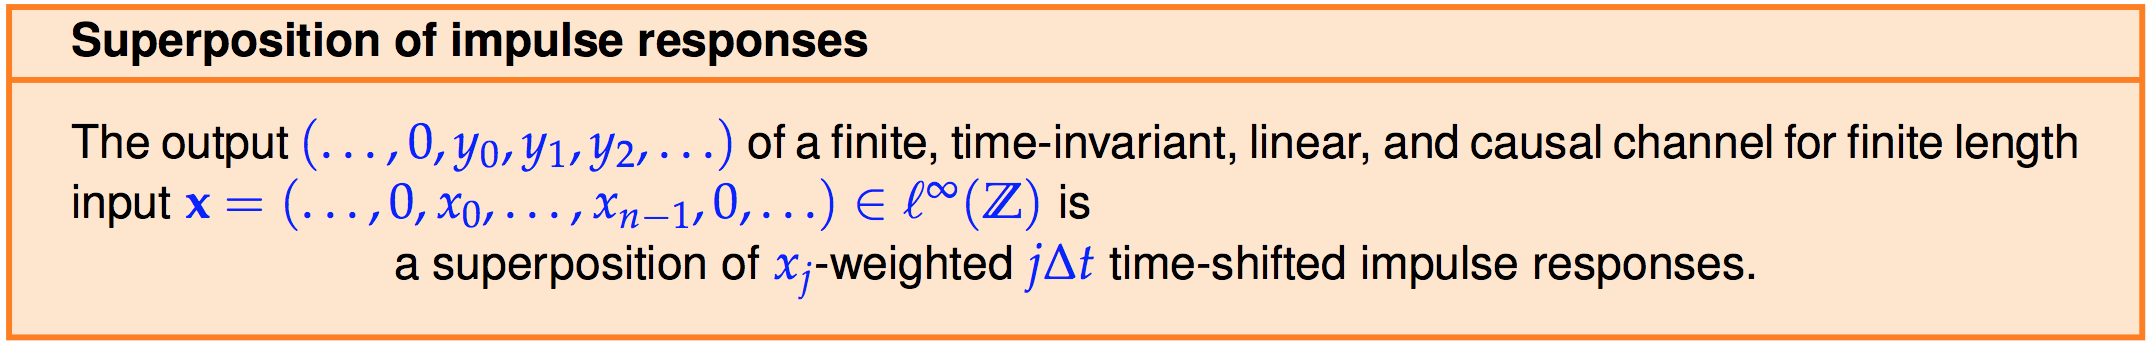
\includegraphics[width=380pt]{superposOfImpulseResp.png}
\end{center}
\subsection{Discrete Convolution}
\begin{center}
	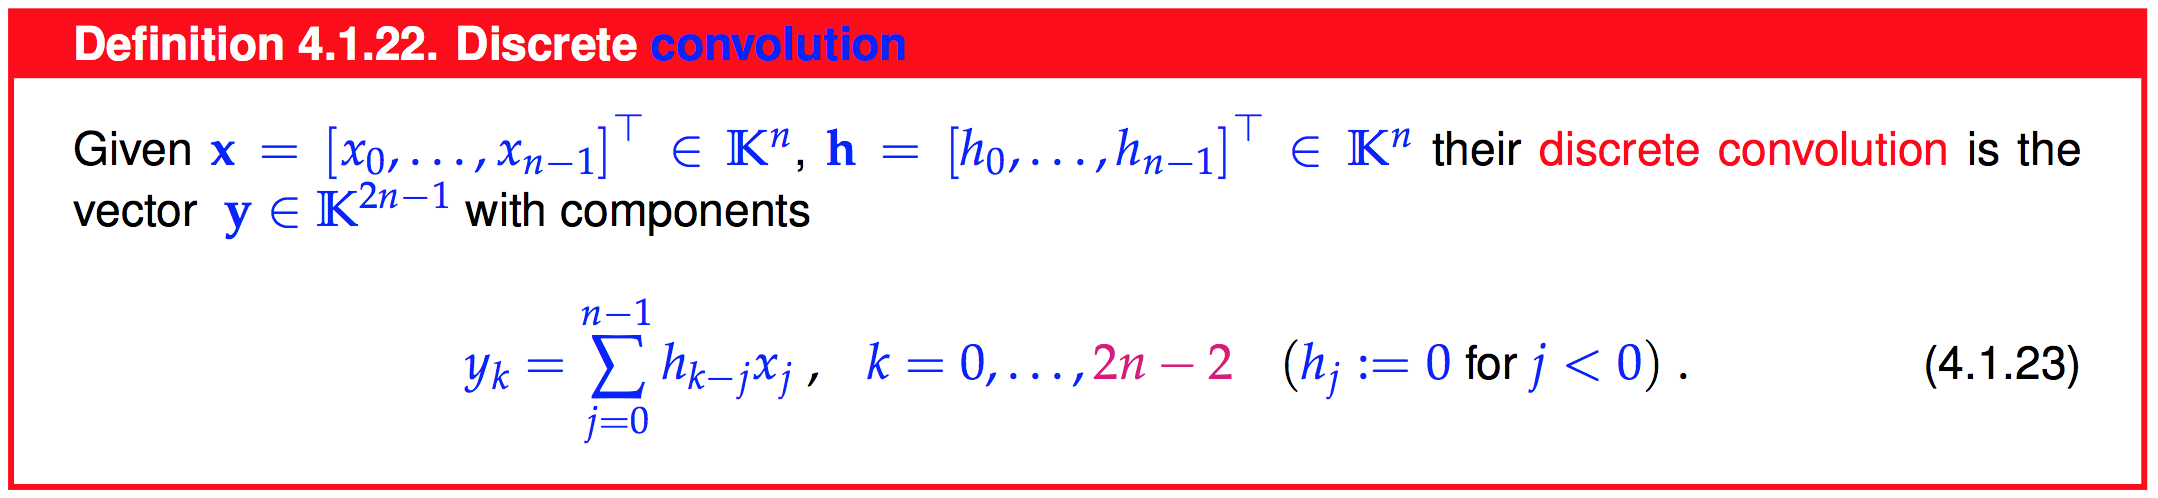
\includegraphics[width=380pt]{DescreteConvolution.png}
\end{center}
A periodic sequence is a sequence satisfying: $x_{j+n} = x_j$, a n periodic sequence will result into a mapping with a n circulant matrix.
\begin{center}
	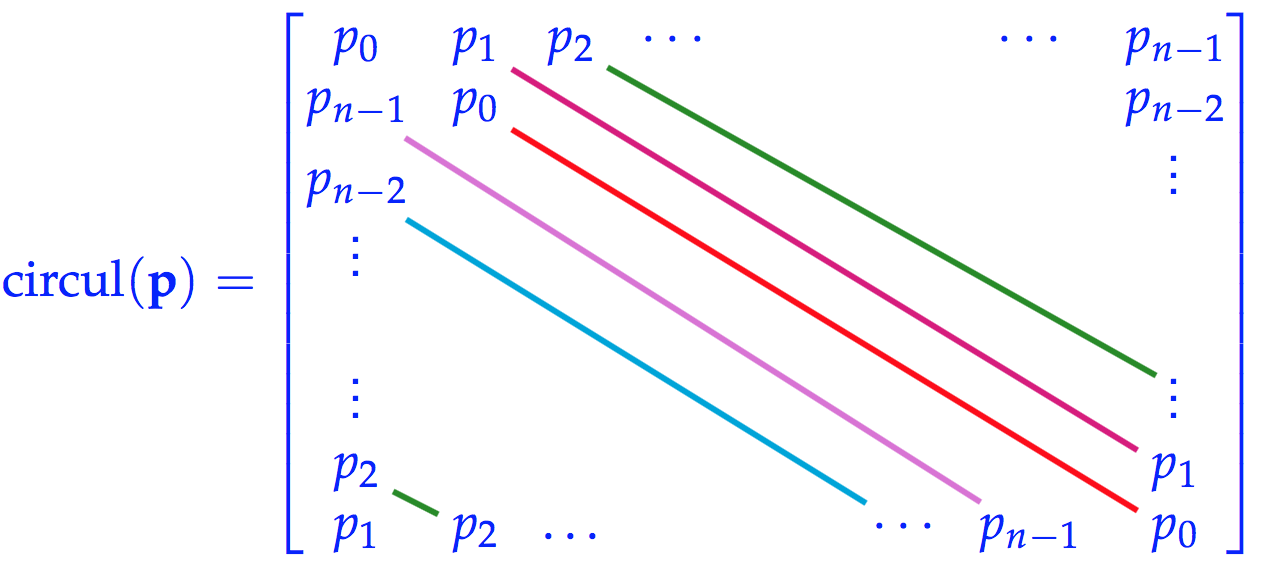
\includegraphics[width=380pt]{circulantMatrix.png}
\end{center}
Discrete convolution can be realized by multiplication with a circulant matrix.\\
Different random circulant matrices have the same eigenvectors!
\subsection{Discrete Fourier Transform (DFT)}
AB = BA, and A has n distinct eigenvalues, then the eigenspaces of A and B coincide.
\begin{center}
	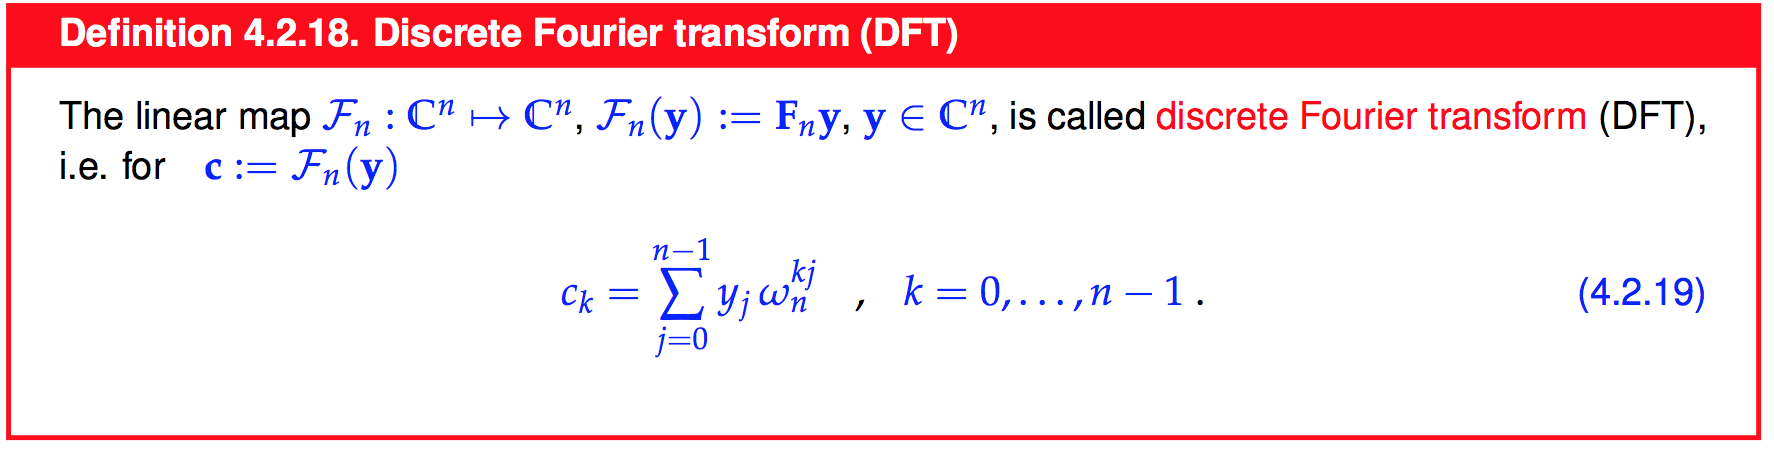
\includegraphics[width=380pt]{dft.png}
\end{center}
\paragraph{Convolution with DFT}
\begin{center}
	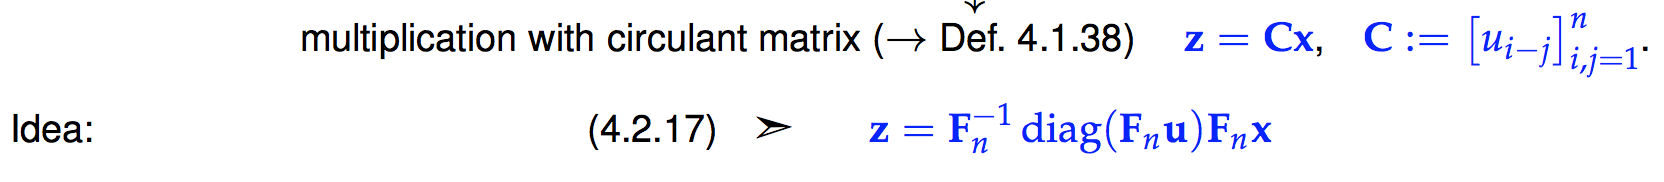
\includegraphics[width=380pt]{convDFT.png}
\end{center}

\section{Quadrature}

\subsection{Error Estimates}

The \textbf{asymptotic decay} of the quadrature error for $n$-point \textbf{Gauss-Legendre} and \textbf{Clenshaw-Curtis} quadrature behaves as follows:
\begin{equation*}
\begin{split}
	f \in C^r([a,b]) & \Rightarrow E_n(f) \rightarrow 0 \quad\textbf{algebraically}\text{ with rate $r$} \\
	f \in C^\infty([a,b]) & \Rightarrow E_n(f) \rightarrow 0 \quad\textbf{exponentially}
\end{split}
\end{equation*}

\emph{Remark:} In order to make an integrand smoother, transform it so that its derivative doesn't have any singularities.

\begin{center}
	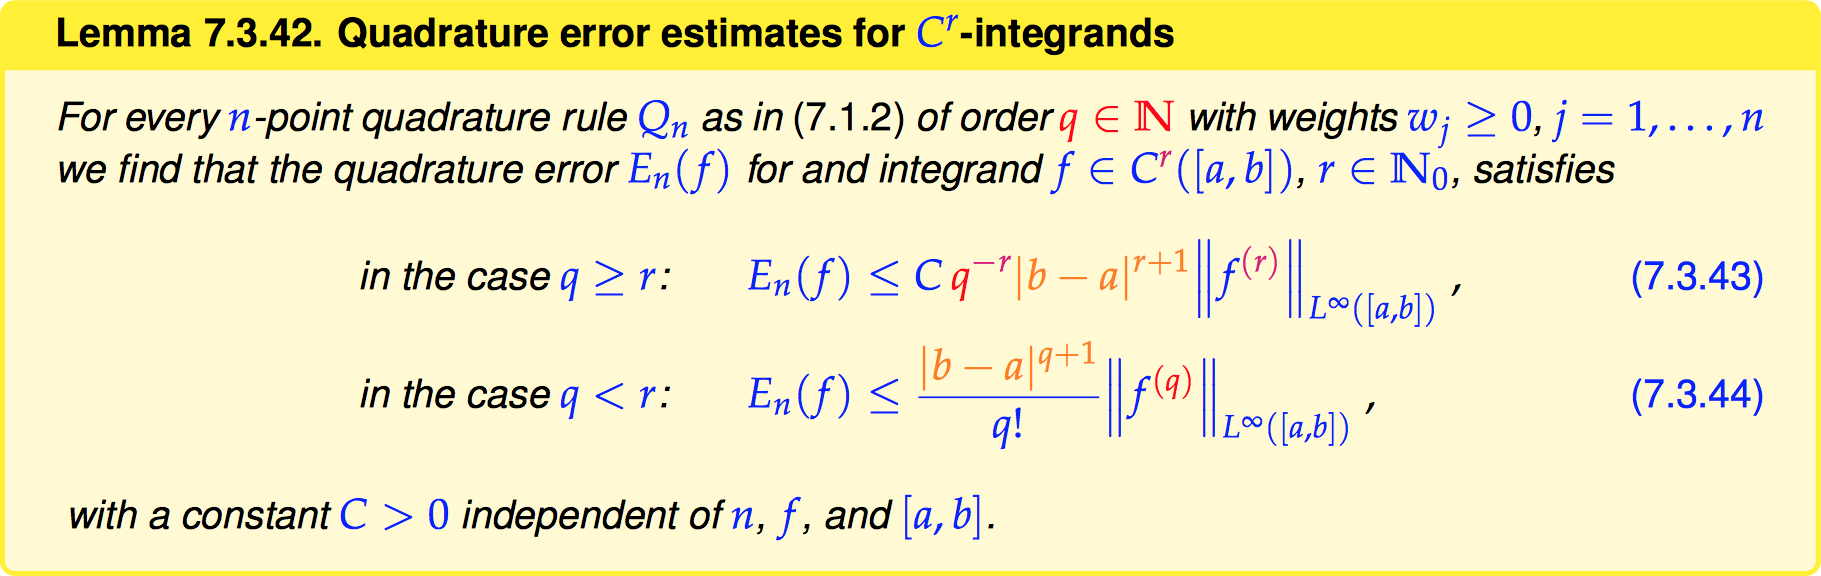
\includegraphics[width=380pt]{quadrature_error}
\end{center}


\end{document}










